\casesection{Uniform sediment}
\label{case:e02-f22-c02}

\paragraph*{To do:}
\begin{itemize}
	\item Fix figures (resize and focus)
	\item Rerun cases
	\item Rerun and add triangle case
\end{itemize}


\paragraph*{Purpose}
The purpose of this validation case is to examine the performance of D-Flow FM-sed-mor in simulating uniform sediment. A straight channel flow simulations with minor longitudinal slope and trench in middle of the channel has been prescribed. The test case reference number is e02-f22-c02.

\paragraph*{Linked claims}
The uniform sediment simulation in module performs well, according to the comparison executed between two simulations (with structured, unstructured FM grid and curvilinear grid of Delft3D) of the test case.

\paragraph*{Approach}
Three simulations have been prepared
and all the input is specified using D-Flow flexible mesh (FM)-sed-mor module.

\paragraph*{Model Description}
In this test case  we use a network of straight channel. A straight channel flows with a constant roughness factor under equilibrium flow conditions. A discharge $Q$ of 0.09945 m$^3$/s is prescribed as an upstream boundary condition. The longitudinal bottom slope $i_b$ is prescribed to be 0.012 (see figure \ref{fig:C02a} and \ref{fig:C02b} ). The length of the channel is 30~m, while the width of the channel is 0.5~m. The Nikuradse roughness height is set to 0.025~m and evaluated using the White-Colebrook formula. The downstream boundary condition is water level set to 0~m.

In this test-case a uniform sediment grain size $D_{50} = 1.4 \cdot 10^{-4}$ is used. 

The default parameters in the morphological setup are mainly used. Nevertheless, in the following section important related setup of morphology and sediment files used are described as follows:
\begin{itemize}
	\item[$\bullet$] Sediment file $<*.sed>$:
\end{itemize}
\begin{verbatim}
[Sediment]
Name             = #Sediment sand#               Name of sediment fraction
SedTyp           = sand                          Must be "sand", "mud" or "bedload"
RhoSol           =  2.6500000e+003      [kg/m3]  Specific density
SedDia           =  1.4000000e-004      [m]      Median sediment diameter (D50)
CDryB            =  1.6000000e+003      [kg/m3]  Dry bed density
IniSedThick      =  5.0000000e-001      [m]      Initial sediment layer thickness at bed (uniform value or filename)
FacDSS           =  1.0000000e+000      [-]      FacDss * SedDia = Initial suspended sediment diameter. Range [0.6 - 1.0]
TraFrm           = 1
ACAL             = 1.0
\end{verbatim}

Sediment transport equation is the transport relation by \cite{EngelundH67}).
\begin{itemize}
	\item[$\bullet$] Morphology file $<*.mor>$:
\end{itemize}
The morphological update $MorUpd$ and bed composition update  $CmpUpd$ are switched off to check the bed load transport. Then it is swithed on to check the bed level change. $MorFac$ is equal to 18 and the spin-up interval from the start time until the start of morphological changes $MorStt$ is 5.0 minutes.

Two models of FM are set up one with structured grid and the second model with unstructured grid. The results of the bed load transport along channel centerline are compared with Delft3D as shown in figure \ref{fig:mag}.The direction of the bed load transport of the three simulations are compatible as shown in \ref{fig:Vec0}.
Furthermore, two models of FM are set up one with structured grid and the second model with unstructured grid. The results of the bed change along channel centerline are compared with Delft3D as shown in figure \ref{fig:bed}.
\begin{figure}[h!]
	\begin{center}
		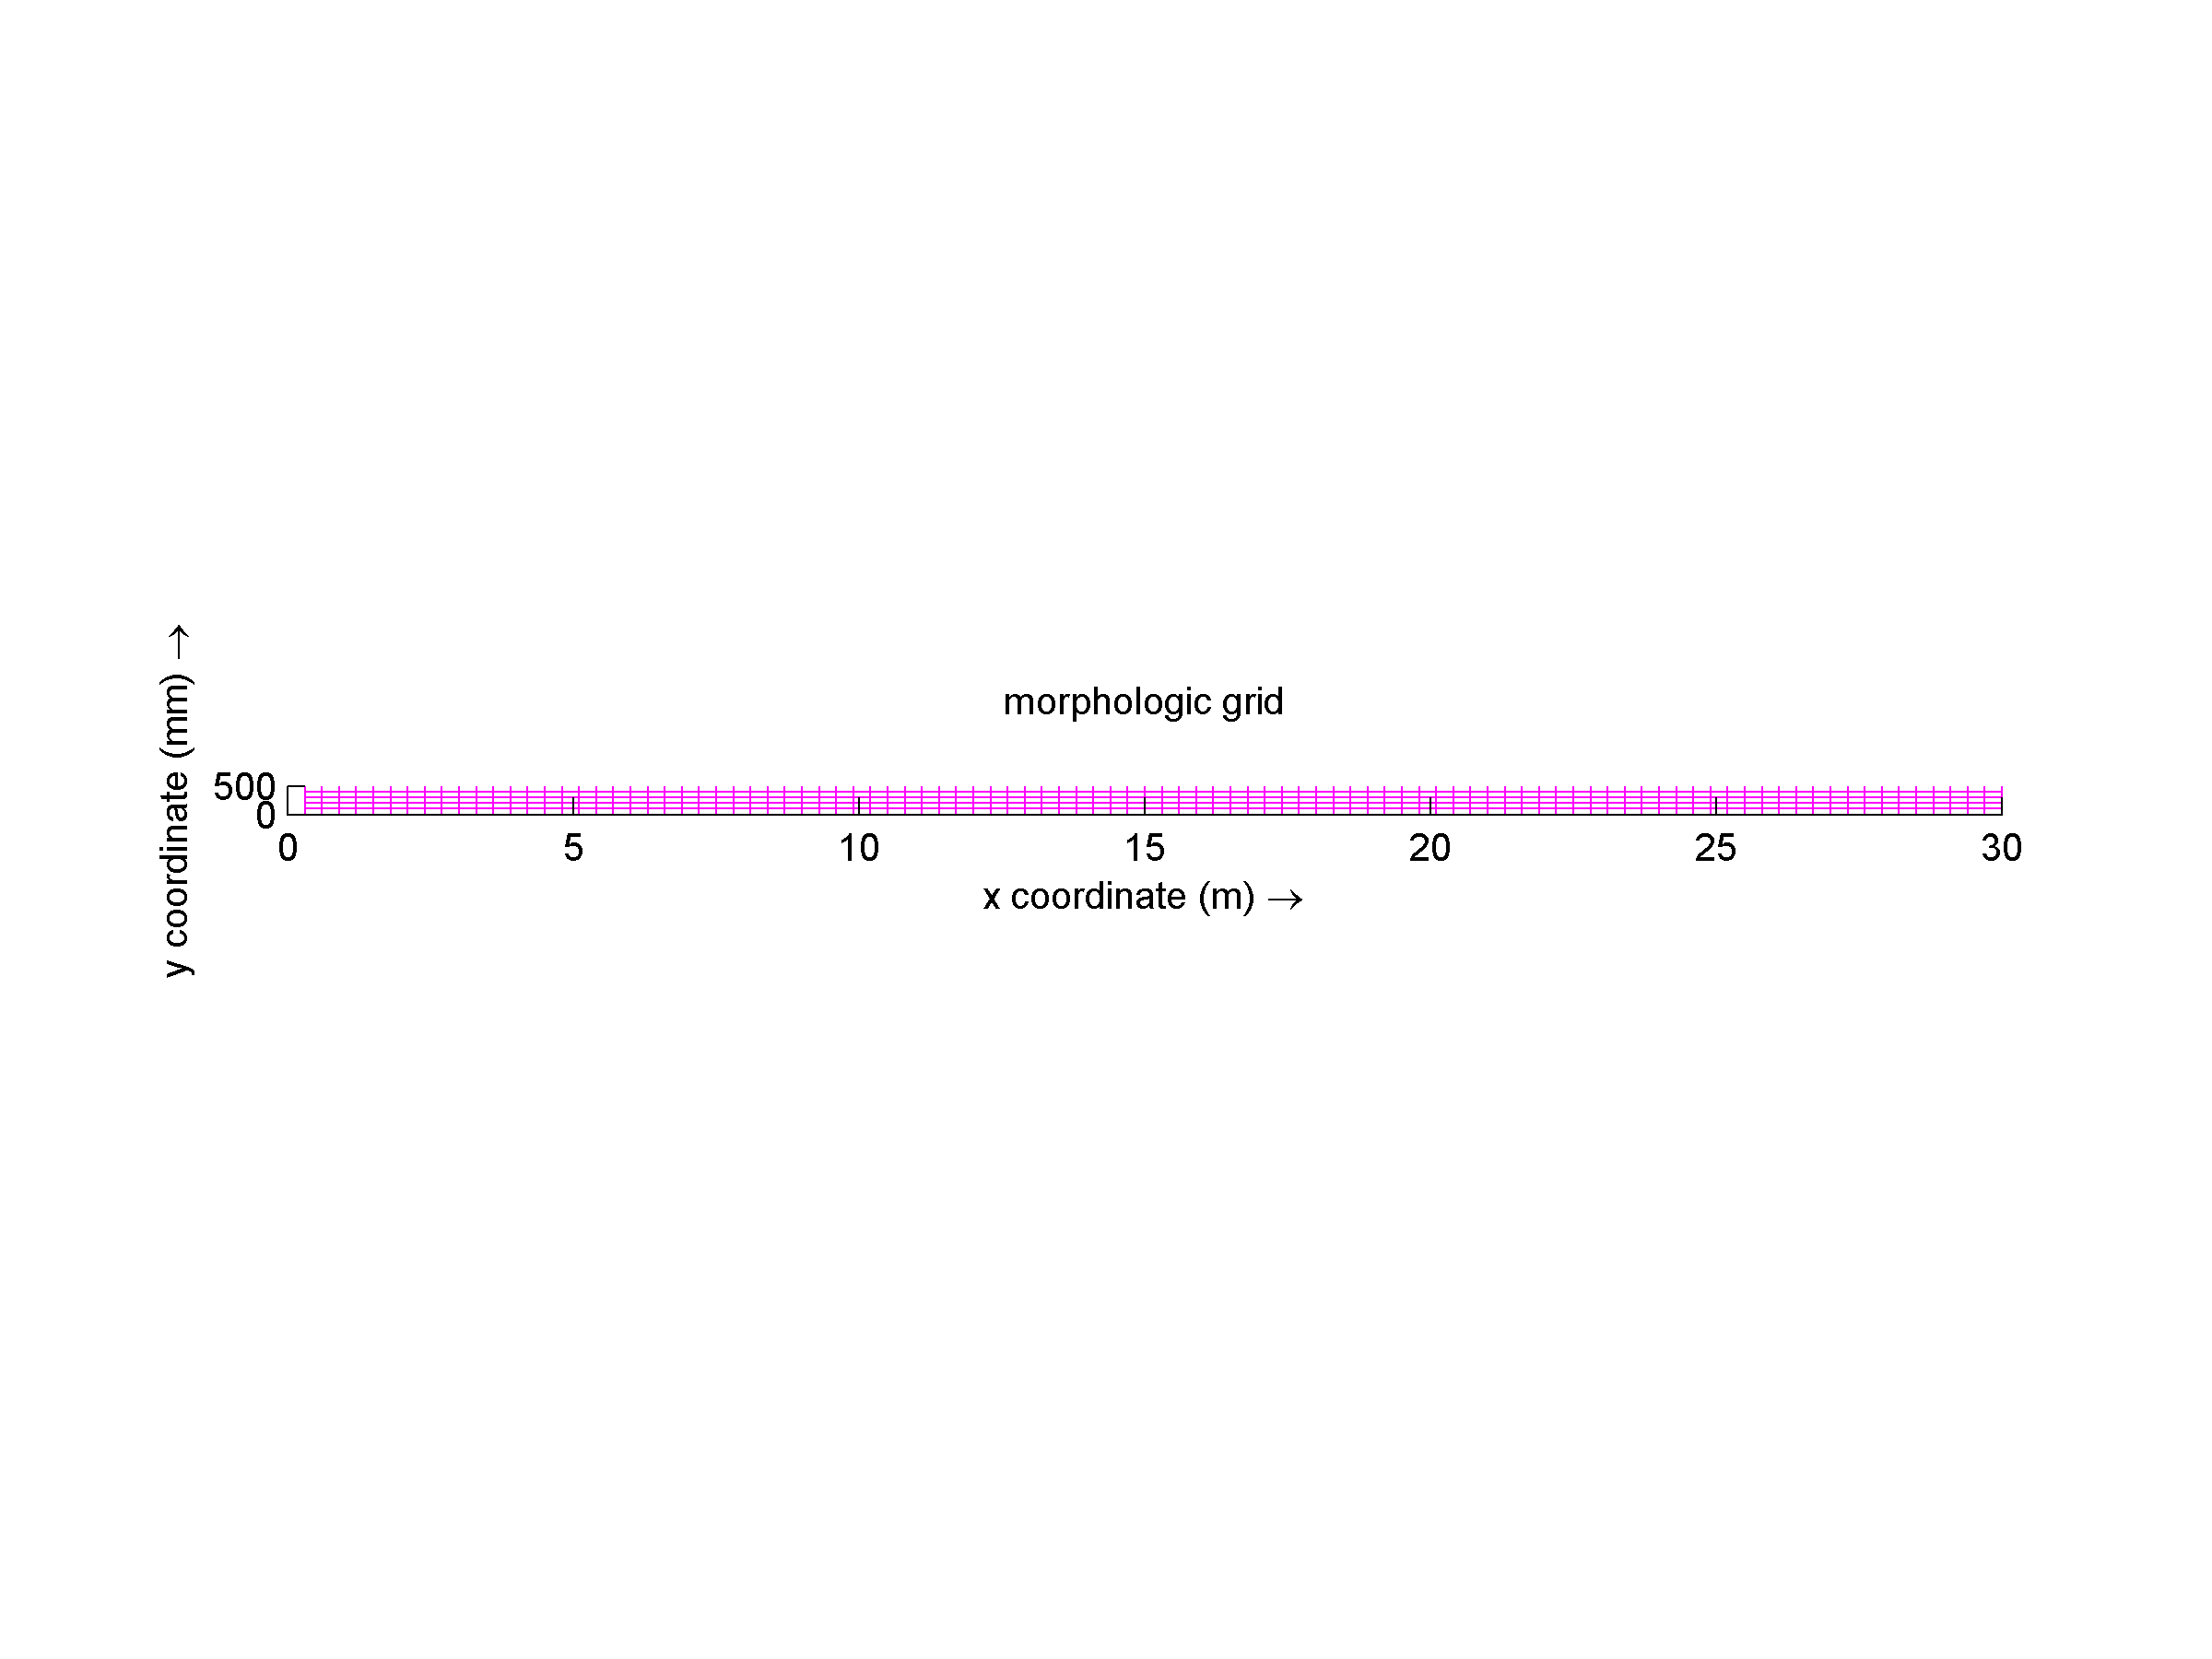
\includegraphics[width=1\columnwidth] {figures/fmnet.png}
	\end{center}\caption{Structured Grid used}
	\label{fig:C02a}
\end{figure}
\begin{figure}[h!]
	\begin{center}
		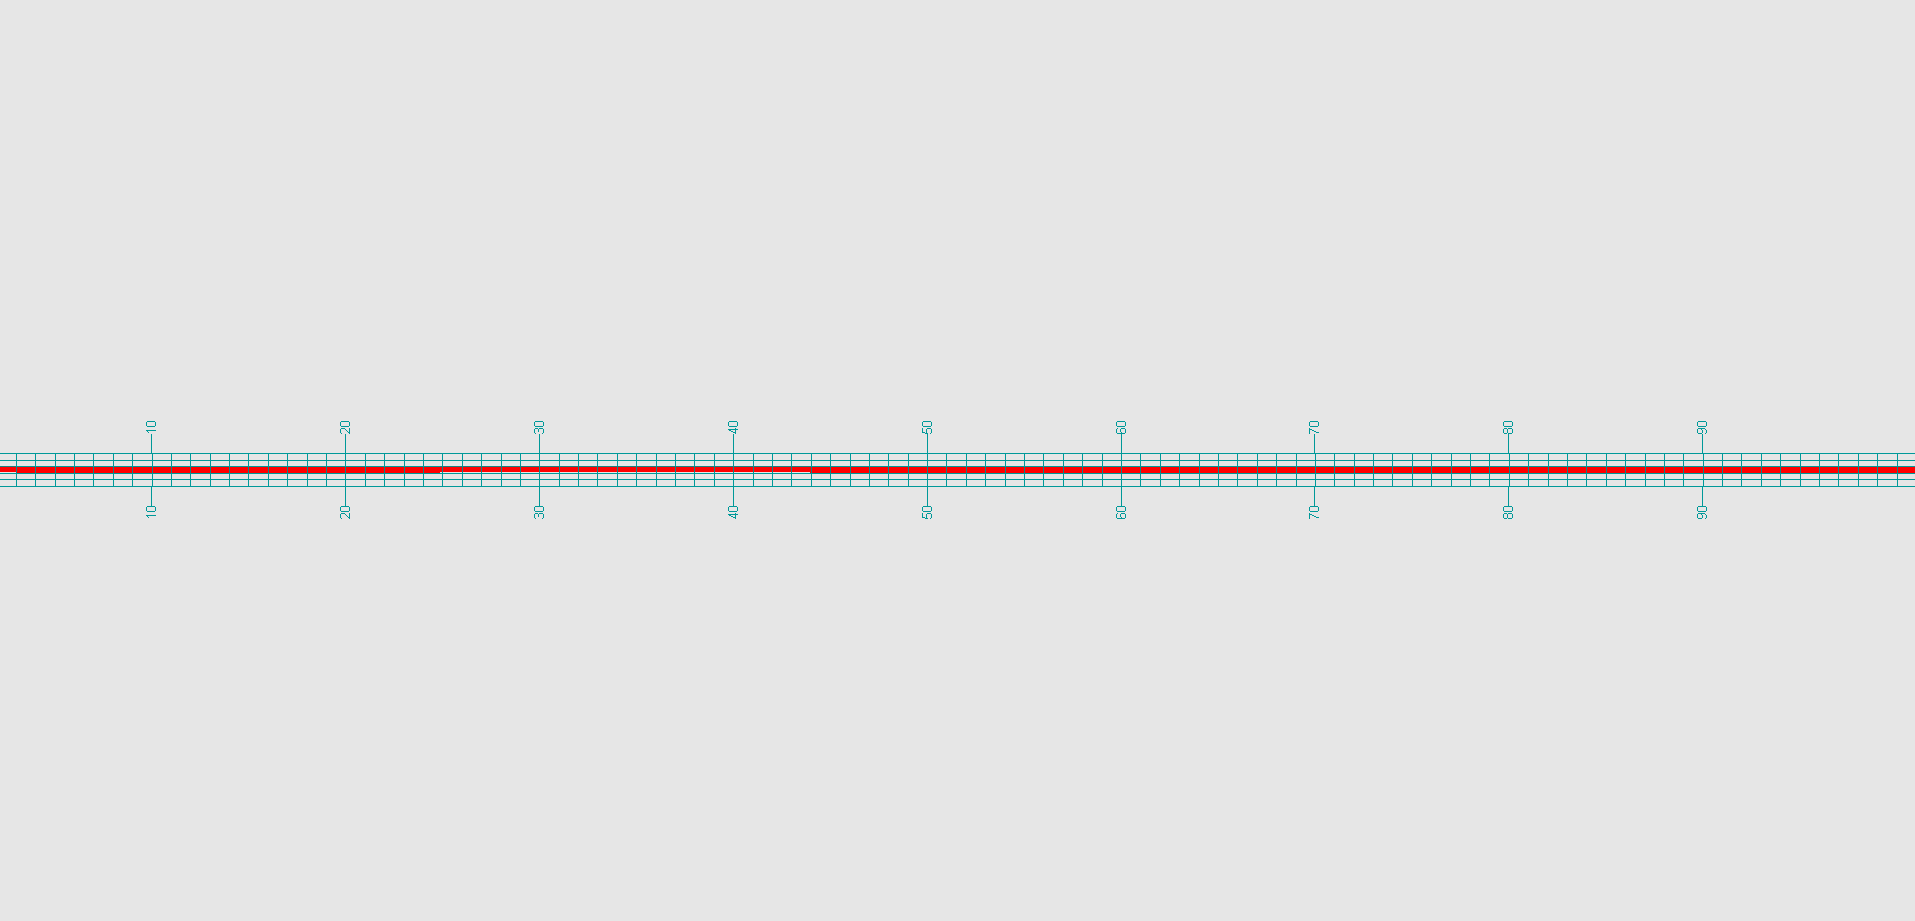
\includegraphics[width=0.7\columnwidth] {figures/centerline.PNG}
	\end{center}\caption{The longitudinal section of the centerline}
	\label{fig:long}
\end{figure}

\begin{figure}[h!]
	\begin{center}
		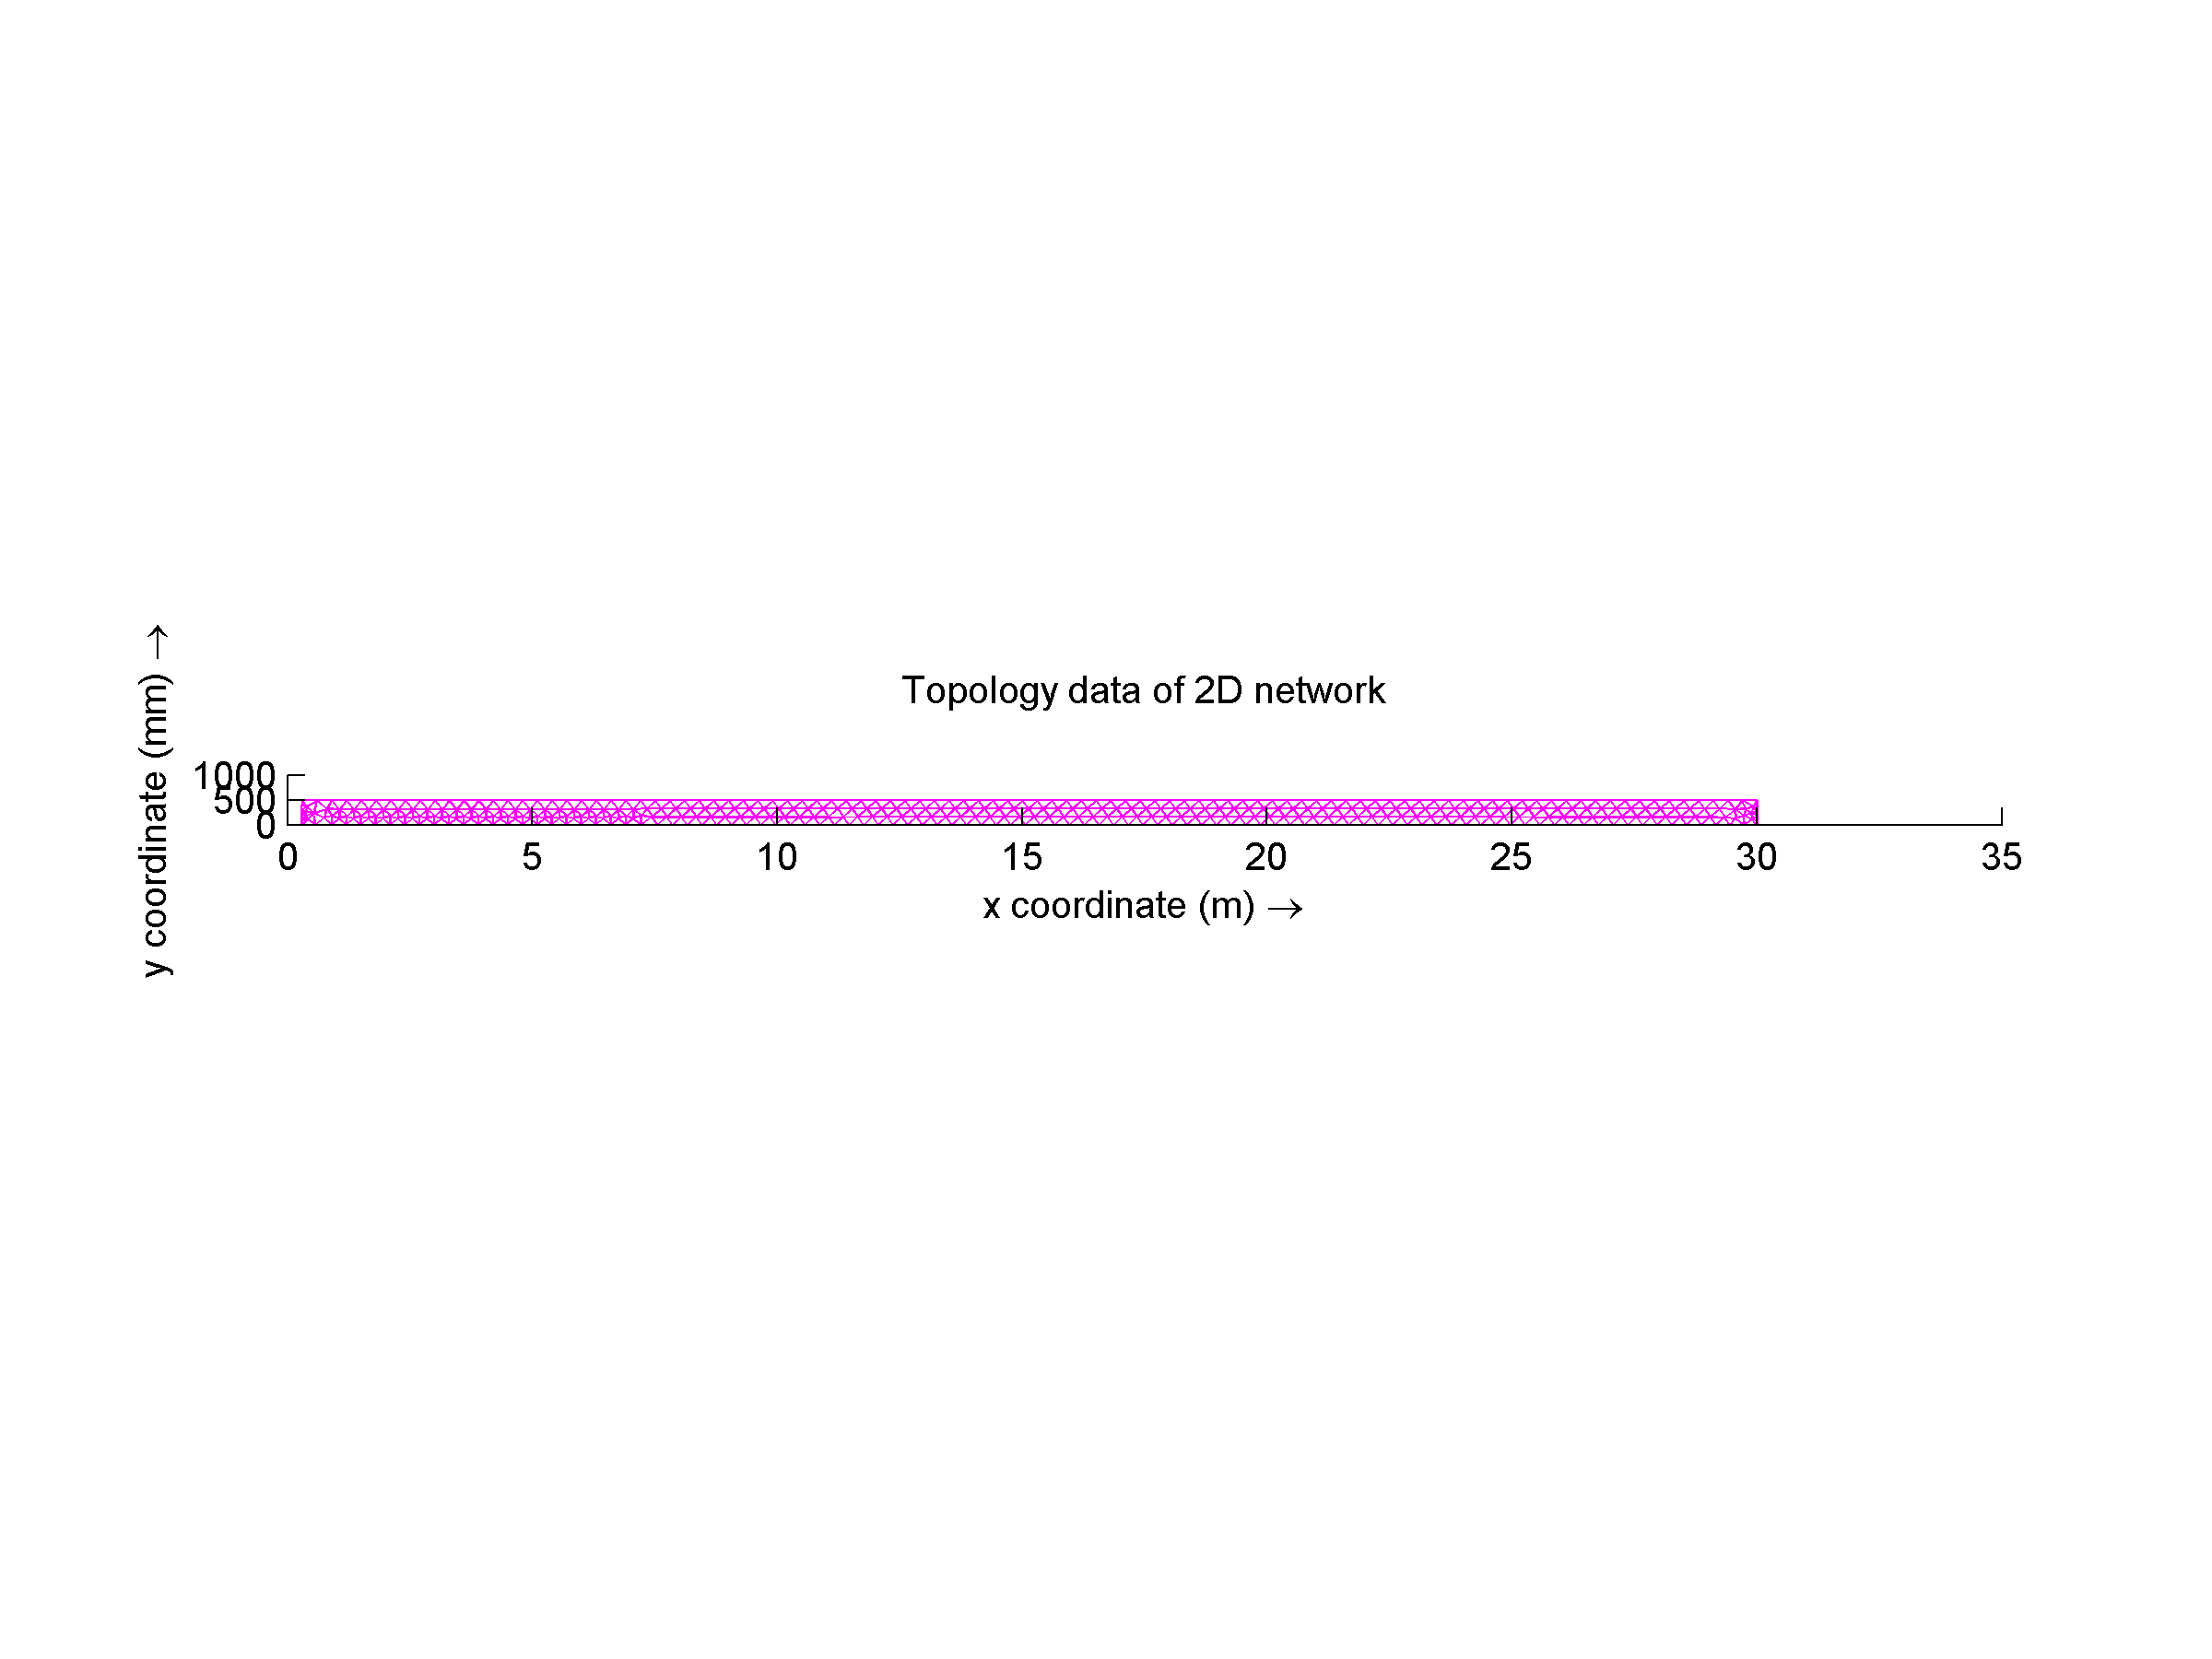
\includegraphics[width=0.7\columnwidth] {figures/fmunstr-net.png}
	\end{center}\caption{Unstructured Grid used}
	\label{fig:C02b}
\end{figure}

\begin{figure}[h!]
	\begin{center}
		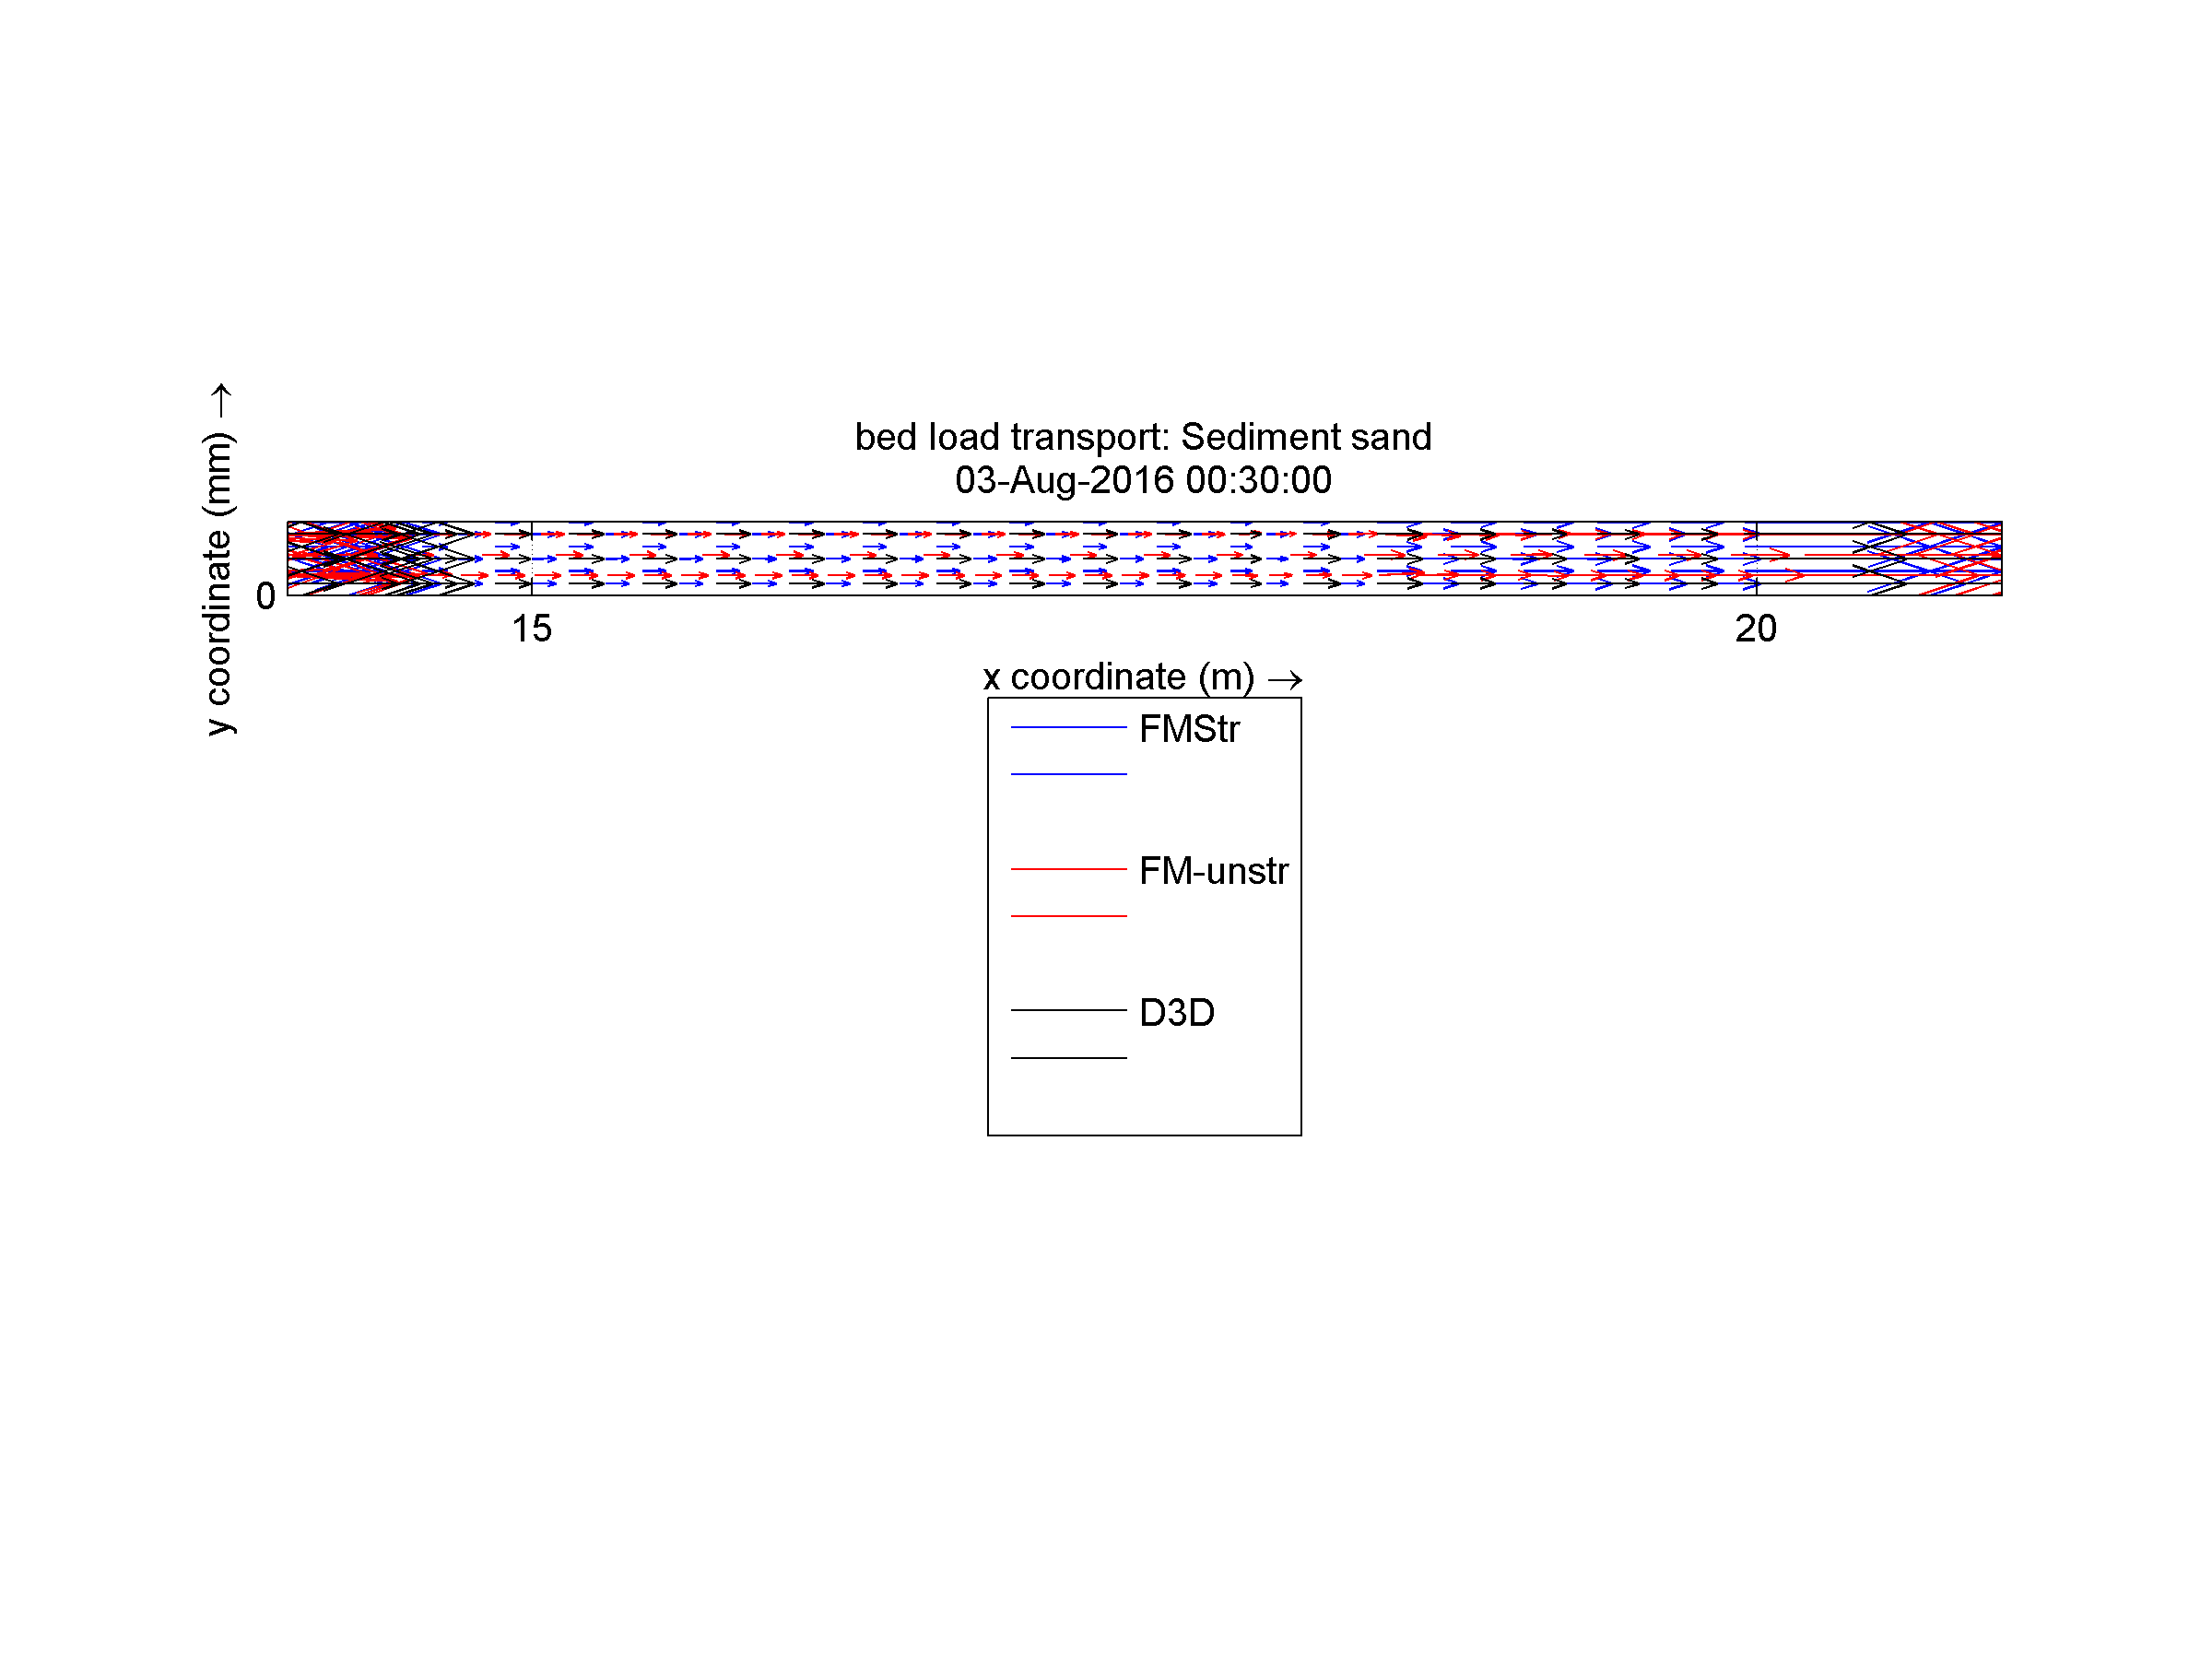
\includegraphics[width=0.7\columnwidth] {figures/C02-Uniform-sediment-VectorMap.png}
	\end{center}\caption{Bed load transport direction at the middle of the model domain}
	\label{fig:Vec0}
\end{figure}

\begin{figure}[h!]
	\begin{center}
		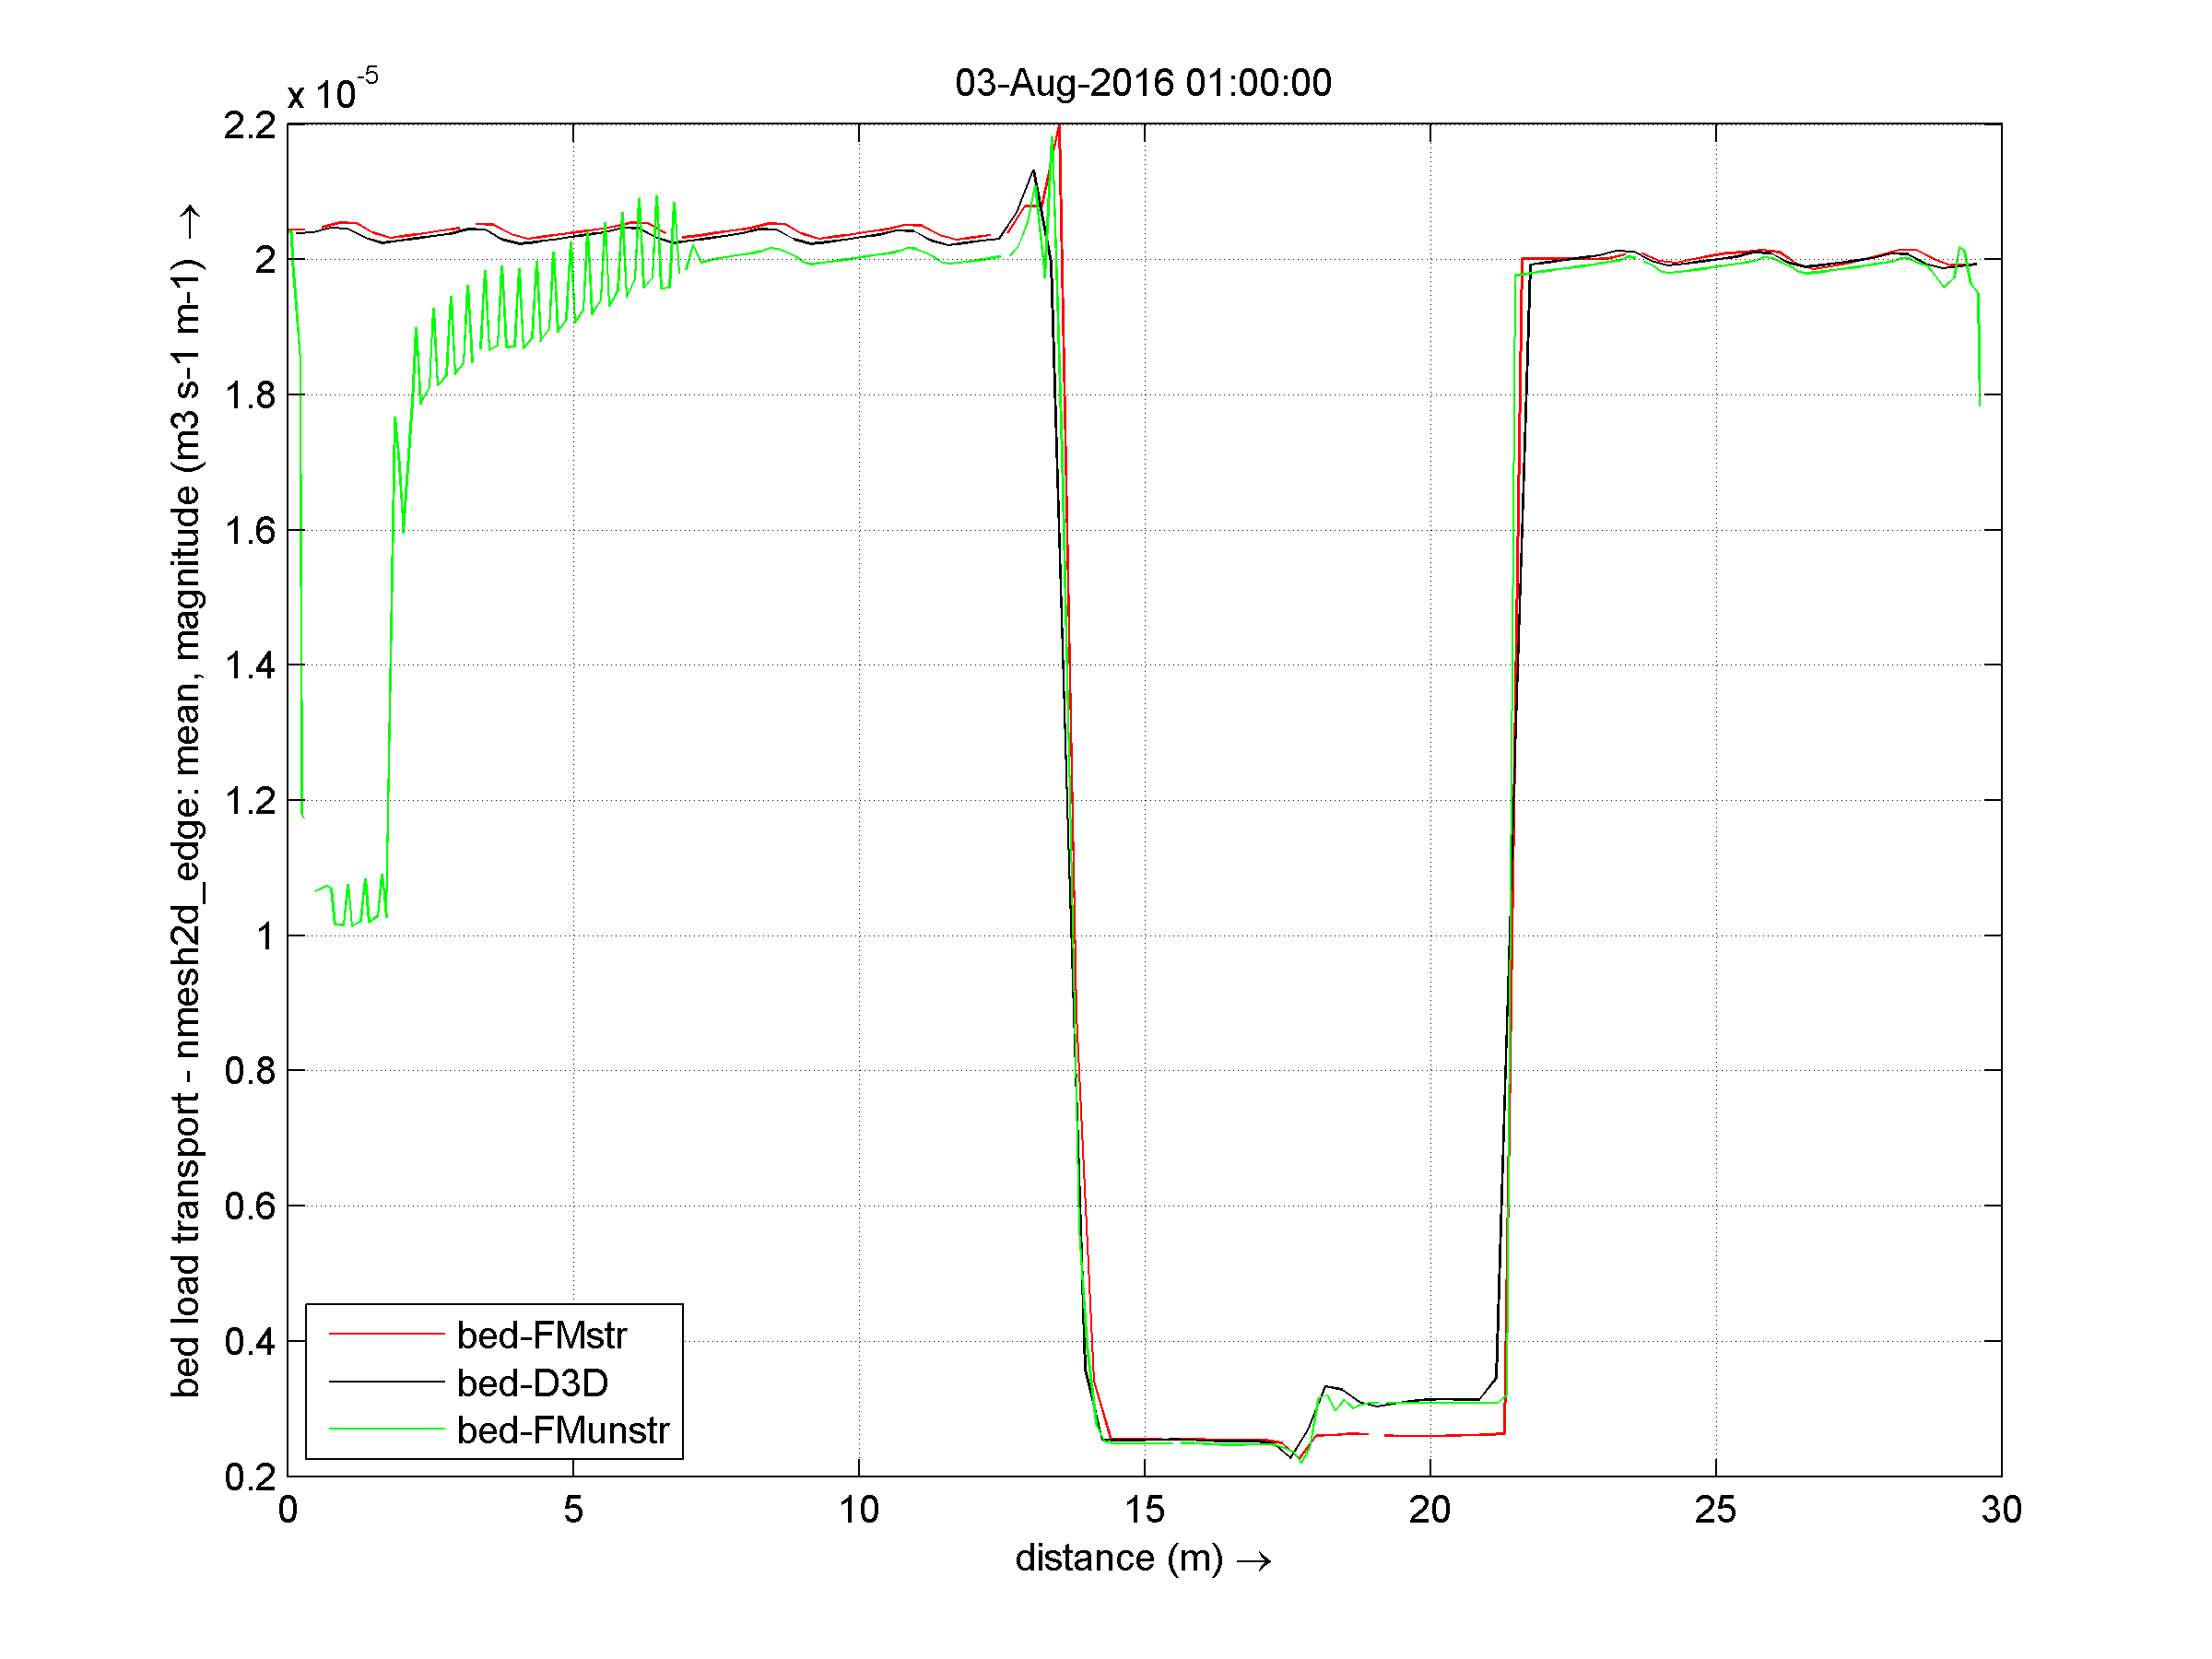
\includegraphics[width=0.7\columnwidth]{figures/C02-bedloadTransport.png}
	\end{center}\caption{Bed load transport magnitude along the centerline of the model domain}
	\label{fig:mag}
\end{figure}

\begin{figure}[h!]
	\begin{center}
		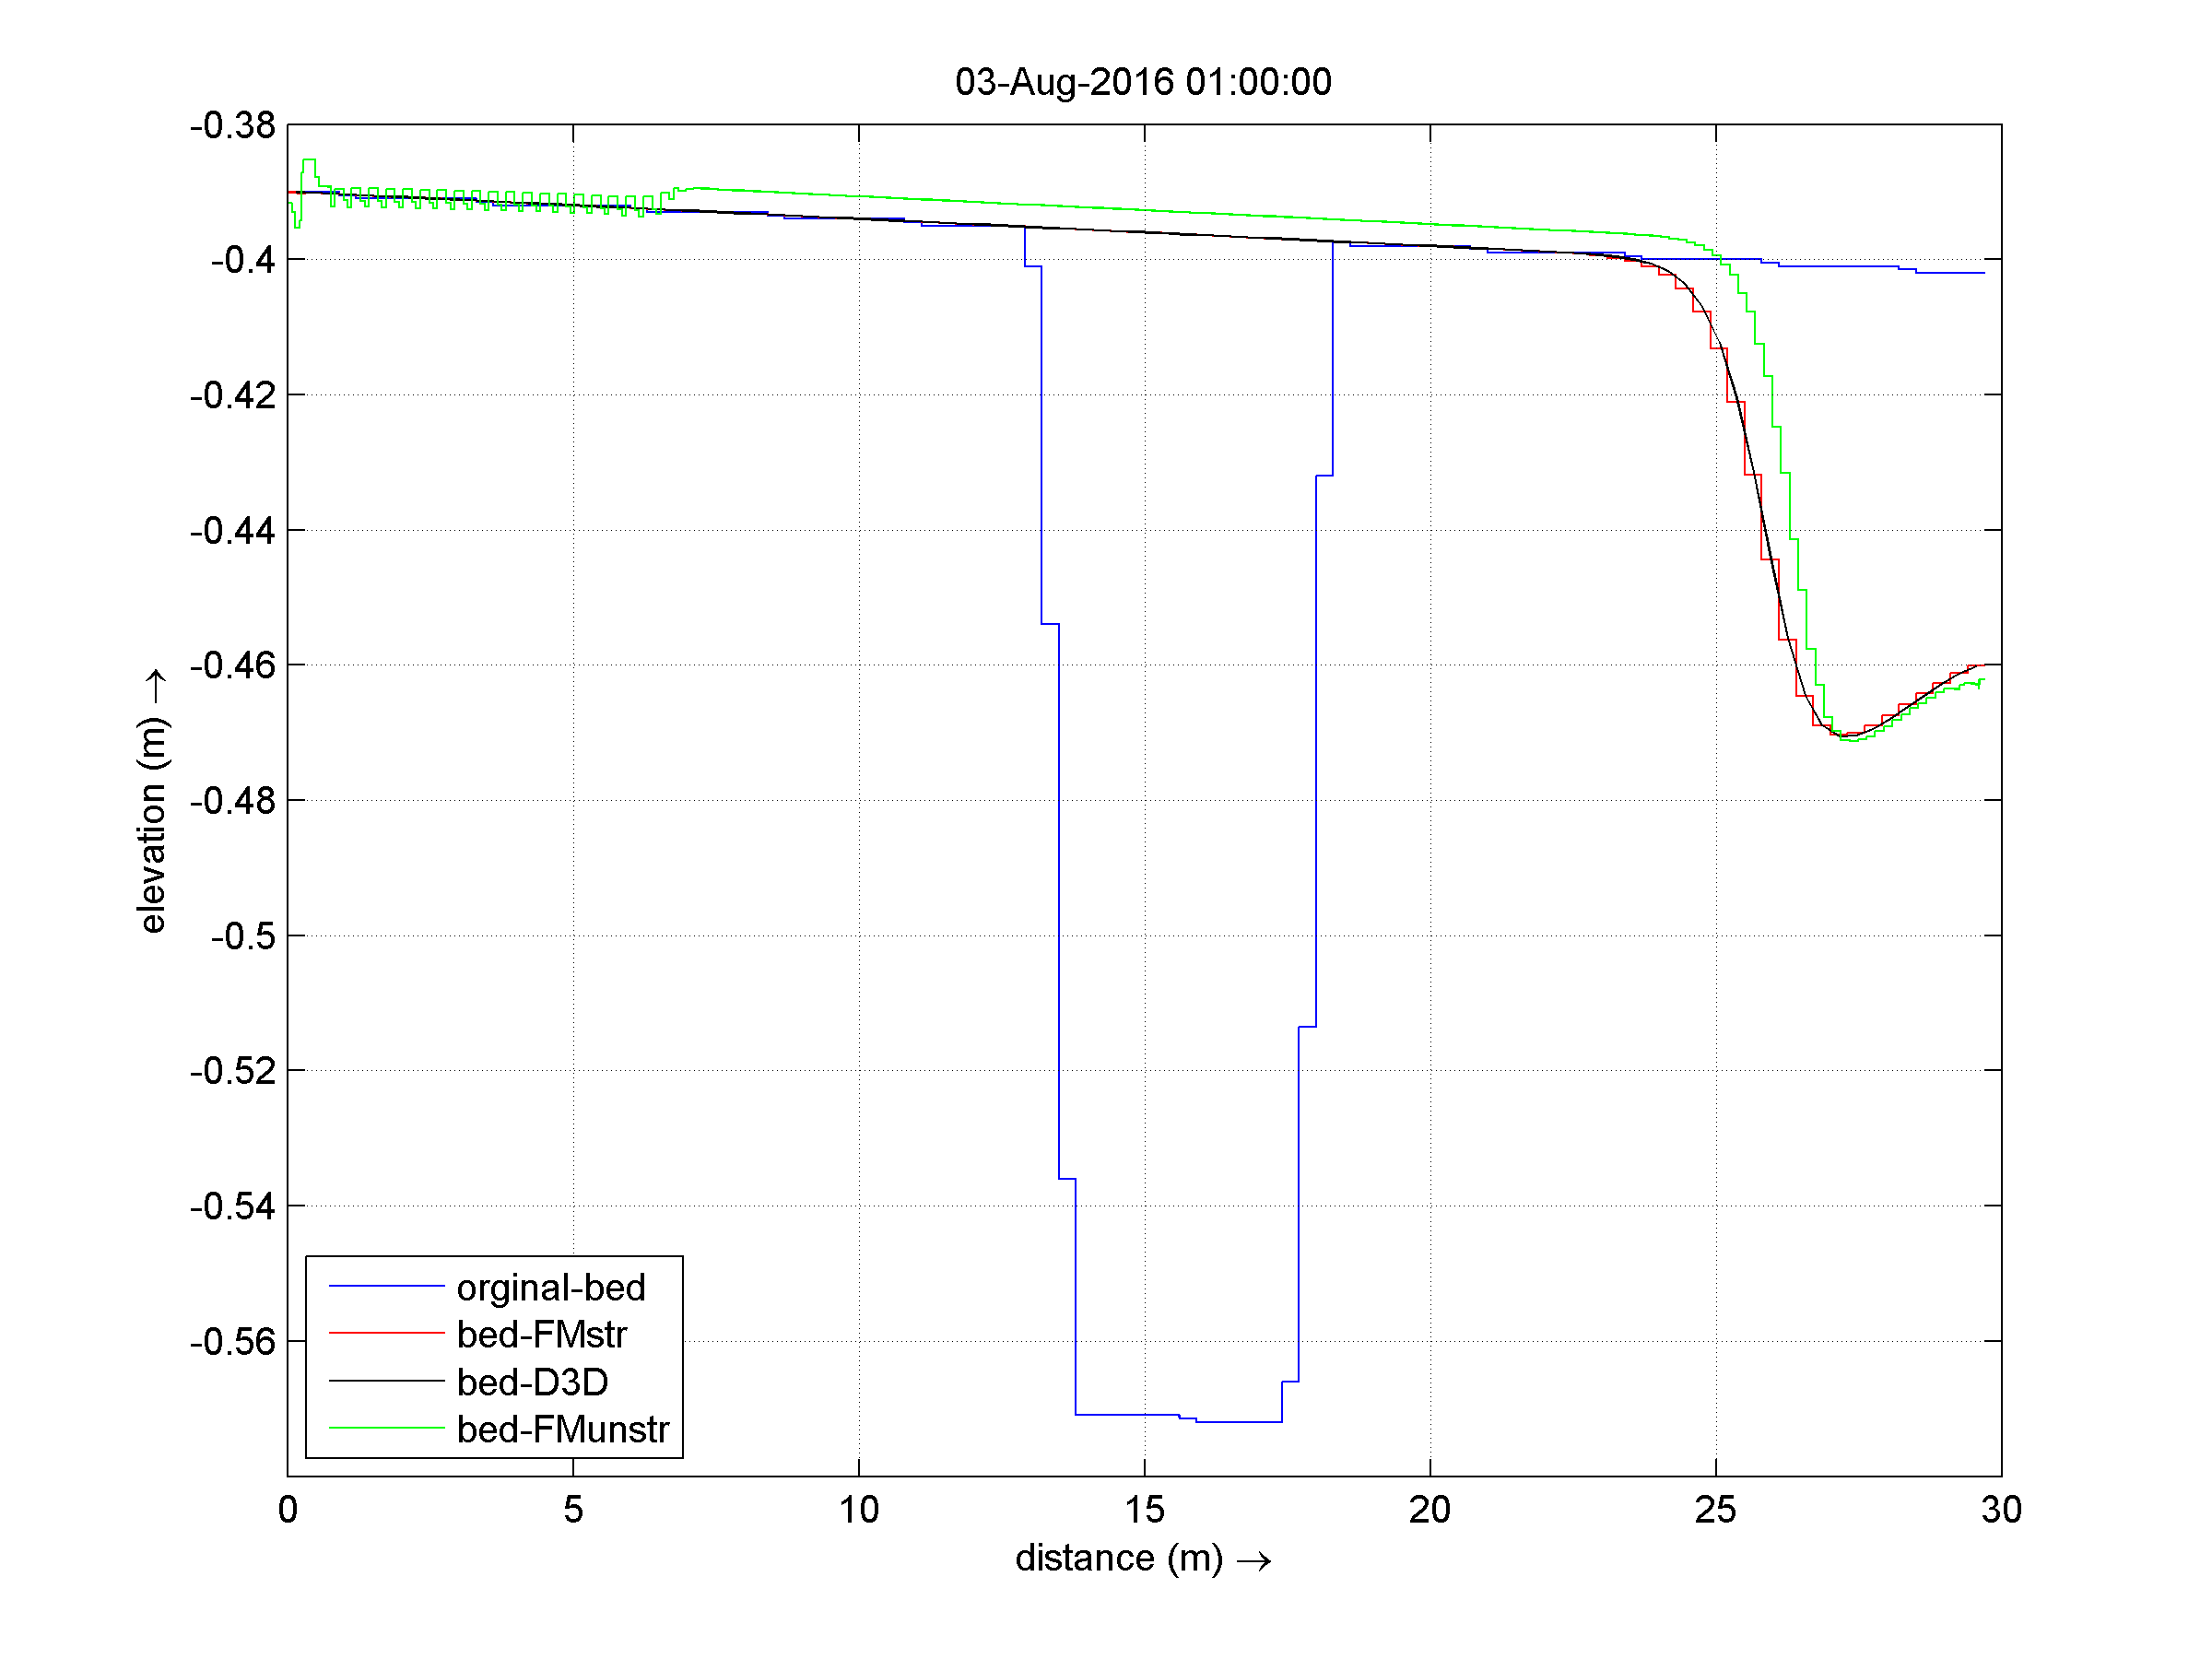
\includegraphics[width=0.7\columnwidth] {figures/C02-bedComparisonv1.png}
	\end{center}\caption{The bed level change along the centerline of the channel}
	\label{fig:bed}
\end{figure}


\paragraph*{Results}

The results that the structured grid produces similar behavior in the transport and bed change as Delft3D4. However, the unstructured grid deviated a bit from them as shown in figure \ref{fig:mag} and \ref{fig:bed}

\paragraph*{Conclusion}
The result shows that uniform sediment work well in FM (Sed-mor) structured grid. The unstructured grid is not gives the exact behavior but it is compatible.
\paragraph*{Version}
This test has been carried out with the following software versions:
\begin{itemize}
	
	\item[$\bullet$] DFLOWFM, dflow-fm-x64-1.1.188.47116
	\item[$\bullet$] Delft3D 4, FLOW2D3D Version 6.02.07.6118
	
\end{itemize}

\paragraph*{References}
\begin{thebibliography}{1}
	
	\bibitem[{Engelund and Hansen (1967)}]{EngelundH67}
	Engelund, F. and Hansen, E., 1967, A monograph on Sediment Transport in Alluvial Streams. Teknisk Forlag, Copenhagen.
	
\end{thebibliography}



%------------------------------------------------------------------------------
